%% LyX 2.2.3 created this file.  For more info, see http://www.lyx.org/.
%% Do not edit unless you really know what you are doing.
\documentclass[9pt,twocolumn,english]{article}
\usepackage[T1]{fontenc}
\usepackage[utf8]{inputenc}
\usepackage{fancyhdr}
\usepackage{graphicx}
\usepackage{amsmath}
\usepackage{geometry}
%%%%% GENEXAMS SPECIFIC %%%%%%%%%%%%
%\mathcode`,="002C
\usepackage{tabularx}
\geometry{verbose,tmargin=1cm,bmargin=2cm,lmargin=1cm,rmargin=1cm}
\usepackage{xcolor,colortbl}
\definecolor{black}{rgb}{0,0,0}
\newcommand{\black}{\cellcolor{black}}  %{0.9}

\makeatletter
%%%%%%%%%%%%%%%%%%%%%%%%%%%%%% User specified LaTeX commands.
\usepackage{setspace}
\usepackage[sort]{cite}
%\pagestyle{empty}
\pagestyle{fancy}
\fancyhead{}
\fancyfoot{}
\renewcommand{\headrulewidth}{0.0pt}
\fancyfoot[RO,RE]{1/2022.12.28-17.37.59}

\makeatother

\usepackage{babel}
\begin{document}

\textbf{University/College/School Name}

\textbf{Institute Name}

\textbf{Departament Name}

\textbf{Prof. Name}\\

Exam/Test 1 -- Physics 101 -- 01 Jan 2023\medskip{}

\textbf{Any important message to students, if necessary}\medskip{}



1. Mark the true alternative.\\
(a) The result of summing a vector and a scalar is a scalar.\\
(b) A vector multiplied by a scalar results is a vector with different direction.\\
(c) Division between vectors is defined in Mathematics.\\
(d) If $\vec{A}$ and $\vec{B}$ are vectors, then $\vec{A}\times\vec{B}$ is a vector perpendicular to both $\vec{A}$ and $\vec{B}$.\\
(e) Vectors can not be multiplied by scalars.\\

2. Consider the rectangle triangle of the figure below and knowing $\theta=15^{\circ}$, determine $\phi$ \textbf{in rad}.\\
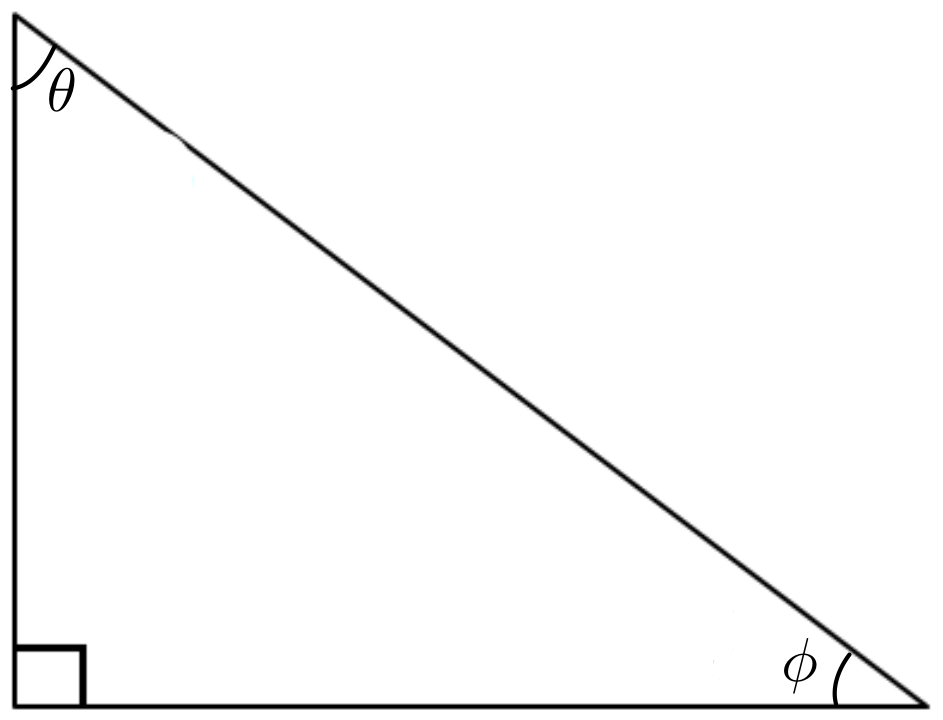
\includegraphics[width=5.0cm]{../input/figs/triangle.png}\\
(a)1.187~
(b)1.309~
(c)1.123~
(d)1.029~
(e)1.278\\

3. A particle of mass 4.4 kg is subject to an external force of 18.3 N. Calculate the acceleration in m/s$^2$ in a one-dimensional movement.\\
(a)7.7~
(b)14.3\\
(c)12.0~
(d)4.2\\
(e)0.3\\


%\noindent\rule{6cm}{0.7pt}\\
{\large \textbf{Fórmulas e Constantes}}
\begin{align*}
%-----------CHAP. 33 and 35-------------
	%&E=E_m\sin(kx-\omega t);~~B=B_m\sin(kx-\omega t)&\\
	%&c=\frac{E}{B}=\frac{E_m}{B_m}={\sqrt{\mu_0 \epsilon_0}};~~\vec{S}=\frac{1}{\mu_0}\vec{E}\times\vec{B}&\\
	%&I=\frac{1}{c\mu_0}\frac{E_m^2}{2};~~I=\frac{P_s}{4\pi r^2};~~P_r=\frac{F}{A}=\gamma\frac{I}{c}~(\mathrm{onde}~1\leq\gamma\leq2)&\\
	%&I=\frac{I_0}{2};~~I=I_0 \cos^2\theta;~~n_1\sin\theta_1=n_2\sin\theta_2~~&\\
	%&\theta_c=\sin^{-1}\frac{n_2}{n_1};~~\theta_B=\tan^{-1}\frac{n_2}{n_1};~~\lambda_n = \frac{\lambda}{n};~~n=\frac{c}{v};~~v=f\lambda&\\
%-----------CHAP. 38 and 39-------------
	&I=\frac{P_s}{4\pi r^2};~~E=hf;~~p=\frac{hf}{c}=\frac{h}{\lambda}&\\
	&hf=K_\mathrm{max}+\Phi;~~\Delta\lambda=\frac{h}{mc}(1-\cos\phi)&\\
	&\frac{d^2\psi}{dx^2}+\frac{8\pi^2 m}{h^2}[E-U(x)]\psi=0&\\
	&T\approx e^{-2bL},~\mathrm{onde}~b=\sqrt{\frac{8\pi^2 m(U_b-E)}{h^2}}&\\
	&E_n=\left(\frac{h^2}{8mL^2}\right)n^2,~\mathrm{para}~n=1,2,3\dots&\\
	&\psi_n(x)=A\sin\left(\frac{n\pi}{L}x\right),~\mathrm{para}~n=1,2,3\dots&\\
	&\Delta x \Delta p = h/2\pi&\\
%--------CONSTANTS----------------------
	&\epsilon_0 = 8,854\times10^{12}~\mathrm{F/m};~~\mu_0 = 1,257\times10^{-6}~\mathrm{H/m}&\\
	&c=3,0\times10^8~\mathrm{m/s};~~h=6,63\times10^{-34}~\mathrm{J/s}=4,14\times10^{-15}~\mathrm{eV.s}&\\
	&hc=1240~\mathrm{eV.nm}&\\
	&\mathrm{Eletron:}~~mc^2 = 511~\mathrm{keV}&\\
%---------------------------------------
\end{align*}
%\rule{6cm}{0.7pt}
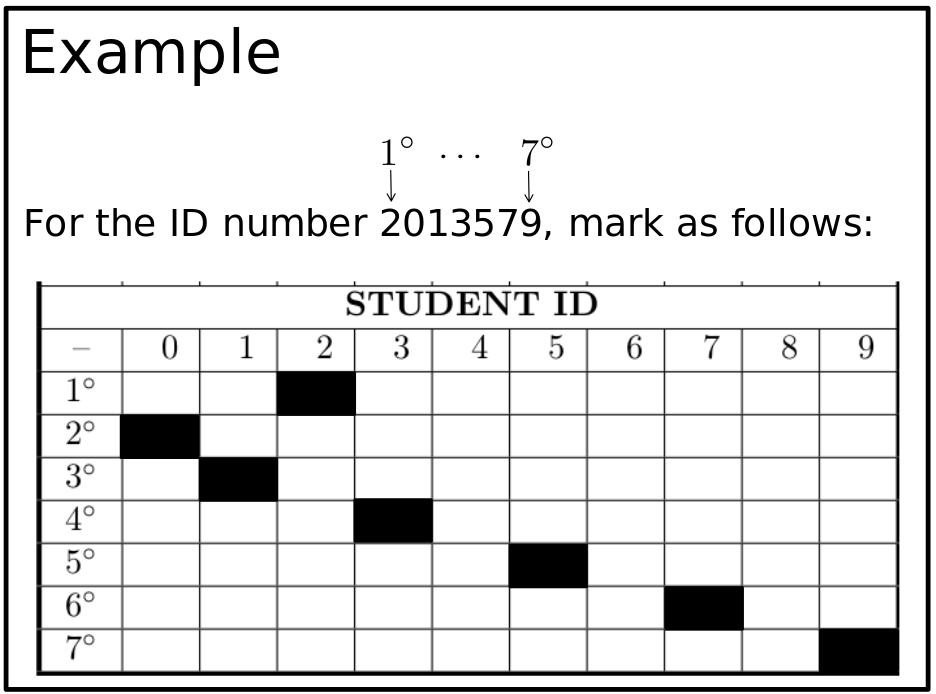
\includegraphics[width=7cm]{../aux/studentidimage_en.png}\\
\vfill
\pagebreak
\begin{tabular}{!{\vrule width 1.5pt}c|c|c|c|c|c|c|c|c|c|c!{\vrule width 1.5pt}}
\noalign{\hrule height 1.5pt}
	\multicolumn{1}{!{\vrule width 1.5pt}c}{} & \multicolumn{9}{c}{\textbf{RESERVED}} & \tabularnewline
\hline 
un&--&\black&--&--&--&--&--&--&--&-- \tabularnewline
\hline%un 
%--&--&--&--&--&--&--&--&--&-- \tabularnewline
 
%--&--&--&--&--&--&--&--&--&--  \tabularnewline
 
	\multicolumn{1}{!{\vrule width 1.5pt}c}{} & \multicolumn{9}{c}{\textbf{ANSWERS}} &  \tabularnewline
\hline
-- & 1 & 2 & 3 & -- & -- & -- & -- & -- & -- & --\tabularnewline
\hline
a &   &   &   & -- & -- & -- & -- & -- & -- & --\tabularnewline
\hline
b &   &   &   & -- & -- & -- & -- & -- & -- & --\tabularnewline
\hline
c &   &   &   & -- & -- & -- & -- & -- & -- & --\tabularnewline
\hline
d &   &   &   & -- & -- & -- & -- & -- & -- & --\tabularnewline
\hline
e &   &   &   & -- & -- & -- & -- & -- & -- & --\tabularnewline
\hline
\multicolumn{1}{!{\vrule width 1.5pt}c}{} & \multicolumn{9}{c}{\textbf{STUDENT ID}} & \tabularnewline
\hline 
-- & \phantom{0}0 & \phantom{0}1 & \phantom{0}2 & \phantom{0}3 & \phantom{0}4 & \phantom{0}5 
& \phantom{0}6 & \phantom{0}7 & \phantom{0}8 & \phantom{0}9\tabularnewline
\hline 
1$^{\circ}$ &  &  &  &  &  &  &  &  &  & \tabularnewline
\hline 
2$^{\circ}$ &  &  &  &  &  &  &  &  &  & \tabularnewline
\hline 
3$^{\circ}$ &  &  &  &  &  &  &  &  &  & \tabularnewline
\hline 
4$^{\circ}$ &  &  &  &  &  &  &  &  &  & \tabularnewline
\hline 
5$^{\circ}$ &  &  &  &  &  &  &  &  &  & \tabularnewline
\hline 
6$^{\circ}$ &  &  &  &  &  &  &  &  &  & \tabularnewline
\hline 
7$^{\circ}$ &  &  &  &  &  &  &  &  &  & \tabularnewline
\noalign{\hrule height 1.5pt}
\end{tabular}
\vfill

\textbf{NAME:}

\vspace{0.5cm}

\textbf{ID NUMBER:}

%\vspace{0.5cm}

%\textbf{TURMA:}
\end{document}